\documentclass[10pt, xcolor=x11names, compress]{beamer}
%\documentclass[10pt, xcolor=x11names, compress, handout]{beamer}
\usetheme{progressbar}
%\usecolortheme[named=Purple4]{structure}
\progressbaroptions{headline=sections,titlepage=normal,frametitle=normal}

\setbeamertemplate{navigation symbols}{}

\usepackage{iwona} 

\usepackage{alltt}
\usepackage{amsmath,amsfonts, amssymb, amscd}
\usepackage{hyperref}
\usepackage{setspace}
\usepackage{wasysym}
\usepackage{ulem}

\usepackage{calc}
\usepackage[overlay,absolute]{textpos}
\TPGrid[5mm,5mm]{20}{20}



\renewcommand{\Re}{\operatorname{Re}}
\renewcommand{\Im}{\operatorname{Im}}
\newcommand{\debye}{\operatorname{debye}}

\newcommand{\chik}{$\chi(k)$}
\newcommand{\chir}{$|\tilde{\chi}(R)|$}


\newcommand{\file}[1]{{\color{Firebrick4}\texttt{`#1'}}}
\newcommand{\multiple}{{\color{Orange3}\textsl{multiple}}}


\newcommand{\atoms}  {{\color{DarkOrchid4}\textsc{atoms}}}
\newcommand{\feff}   {{\color{DarkOrchid4}\textsc{feff}}}
\newcommand{\ifeffit}{{\color{DarkOrchid4}\textsc{ifeffit}}}
\newcommand{\athena} {{\color{DarkOrchid4}\textsc{athena}}}
\newcommand{\artemis}{{\color{DarkOrchid4}\textsc{artemis}}}

\renewenvironment<>{center}
{\begin{actionenv}#1\begin{originalcenter}}
{\end{originalcenter}\end{actionenv}}

\definecolor{guessp}   {rgb}{0.64,0.00,0.64}
\newcommand{\guessp}   {{\color{guessp}guess}}
\definecolor{defp}     {rgb}{0.00,0.55,0.00}
\newcommand{\defp}     {{\color{defp}def}}
\definecolor{setp}     {rgb}{0,0,0}
\newcommand{\setp}     {{\color{setp}set}}
\definecolor{lguessp}  {rgb}{0.24,0.11,0.56}
\newcommand{\lguessp}  {{\color{lguessp}lguess}}
\definecolor{skipp}    {rgb}{0.70,0.70,0.70}
\newcommand{\skipp}    {{\color{skipp}skip}}
\definecolor{restrainp}{rgb}{0.80,0.61,0.11}
\newcommand{\restrainp}{{\color{restrainp}restrain}}
\definecolor{afterp}   {rgb}{0.29,0.44,0.55}
\newcommand{\afterp}   {{\color{afterp}after}}
\definecolor{penaltyp} {rgb}{0.55,0.35,0.17}
\newcommand{\penaltyp} {{\color{penaltyp}penalty}}
\definecolor{mergep}   {rgb}{0.93,0.00,0.00}
\newcommand{\mergep}   {{\color{mergep}merge}}

%% Time-stamp: <2011-10-26 17:01:33 bruce>
%%%%%%%%%%%%%%%%%%%%%%%%%%%%%%%%%%%%%%%%%%%%%%%%%%%%%%%%%%%%%%%%%%%%%%
%%%  Include file for
%%%    A Practical Introduction to Multiple Scattering Theory
%%%                            Copyright (C) 2004-2005, 2011 Bruce Ravel
%%%                            <bravel@anl.gov>
%%%                            http://feff.phys.washington.edu/~ravel
%%%%%%%%%%%%%%%%%%%%%%%%%%%%%%%%%%%%%%%%%%%%%%%%%%%%%%%%%%%%%%%%%%%%%%
%%
%% This work is licensed under the Creative Commons Attribution,
%% Share-Alike License. To view a copy of this license, visit
%% http://creativecommons.org/licenses/by-sa/2.5/ or send a letter to
%% Creative Commons, 559 Nathan Abbott Way, Stanford, California
%% 94305, USA.
%%
%%%%%%%%%%%%%%%%%%%%%%%%%%%%%%%%%%%%%%%%%%%%%%%%%%%%%%%%%%%%%%%%%%%%%%

%%% single scattering
\def  \SS {{
%  \begin{minipage}[h][3truecm][c]{4truecm}
  \begin{picture}(80,26)(0,0)
    \linethickness{1pt}
    \qbezier(8,13)(40,26)(72,13)
    \qbezier(8,13)(40,0)(72,13)
    {\color{red}
    \put(8,13){\circle*{9}}}
    {\color{Gold2}
    \put(72,13){\circle*{9}}}
  \end{picture}
%  \end{minipage}
}}

%%% double scattering
\def  \DS {{
  \begin{minipage}[h][2truecm][c]{3truecm}
  \begin{picture}(125,60)(0,0)
    \linethickness{1pt}
    \qbezier(12.5,20)(25,40)(62.5,50)
    \qbezier(62.5,50)(100,40)(112.5,20)
    \qbezier(12.5,20)(62.5,0)(112.5,20)
    {\color{red}
    \put(12.5,20){\circle*{13}}}
    {\color{blue}
    \put(59,50){\circle*{13}}
    \put(112.5,20){\circle*{13}}}
  \end{picture}
  \end{minipage}
}}

%%% triple scattering #1
\def  \TST {{
  \begin{minipage}[h][2truecm][c]{3truecm}
  \begin{picture}(125,60)(0,0)
    \linethickness{1pt}
    \qbezier(12.5,20)(25,40)(62.5,50)
    \qbezier(62.5,50)(100,40)(112.5,20)
    \qbezier(12.5,20)(50,30)(62.5,50)
    \qbezier(62.5,50)(75,30)(112.5,20)
    {\color{red}
    \put(12.5,20){\circle*{13}}}
    {\color{blue}
    \put(59,50){\circle*{13}}
    \put(112.5,20){\circle*{13}}}
  \end{picture}
  \end{minipage}
}}

%%% triple scattering #2
\def  \TSF {{
  \begin{minipage}[h][2truecm][c]{3truecm}
  \begin{picture}(125,60)(0,-20)
    \linethickness{1pt}
    \qbezier(12.5,20)(25,40)(62.5,50)
    \qbezier(62.5,50)(100,40)(112.5,20)
    \qbezier(62.5,-10)(100,0)(112.5,20)
    \qbezier(12.5,20)(25,0)(62.5,-10)
    {\color{red}
    \put(12.5,20){\circle*{13}}}
    {\color{blue}
    \put(59,50){\circle*{13}}
    \put(112.5,20){\circle*{13}}
    \put(59,-10){\circle*{13}}}
  \end{picture}
  \end{minipage}
}}

%% focussed DS
\def  \FDS {{
  \begin{picture}(80,26)(0,0)
    \linethickness{1pt}
    \qbezier(8,13)(20,26)(40,13)
    \qbezier(8,13)(40,0)(72,13)
    \qbezier(40,13)(56,26)(72,13)
    {\color{red}
    \put(8,13){\circle*{9}}}
    {\color{Gold2}
    \put(36,13){\circle*{9}}}
    {\color{Gold2}
    \put(68,13){\circle*{9}}}
  \end{picture}
}}

%% focussed TS
\def  \FTS {{
  \begin{picture}(80,26)(0,0)
    \linethickness{1pt}
    \qbezier(8,13)(20,26)(40,13)
    \qbezier(40,13)(56,26)(72,13)
    \qbezier(8,13)(20,0)(40,13)
    \qbezier(40,13)(56,0)(72,13)
    {\color{red}
    \put(8,13){\circle*{9}}}
    {\color{Gold2}
    \put(36,13){\circle*{9}}}
    {\color{Gold2}
    \put(68,13){\circle*{9}}}
  \end{picture}
}}

% %  \begin{minipage}[h][1truecm][c]{8truecm}
%   \begin{picture}(250,60)(0,0)
%     \linethickness{1pt}
%     \qbezier(12.5,20)(62.5,40)(125,20)
%     \qbezier(125,20)(187.5,40)(225.5,20)
%     \qbezier(12.5,20)(112.5,0)(225.5,20)
%     {\color{Firebrick4}
%     \put(12.5,20){\circle*{13}}}
%     {\color{blue}
%     \put(125,20){\circle*{13}}
%     \put(225.5,20){\circle*{13}}}
%   \end{picture}
% %  \end{minipage}

% %% focussed TS
% \def  \FTS {{
% %  \begin{minipage}[h][1truecm][c]{8truecm}
%   \begin{picture}(250,60)(0,0)
%     \linethickness{1pt}
%     \qbezier(12.5,20)(62.5,40)(125,20)
%     \qbezier(125,20)(187.5,40)(225.5,20)
%     \qbezier(12.5,20)(62.5,0)(125,20)
%     \qbezier(125,20)(187.5,0)(225.5,20)
%     {\color{Firebrick4}
%     \put(12.5,20){\circle*{13}}}
%     {\color{blue}
%     \put(125,20){\circle*{13}}
%     \put(225.5,20){\circle*{13}}}
%   \end{picture}
% %  \end{minipage}
% }}


%%% Local Variables:
%%% mode: latex
%%% TeX-master: t
%%% End:

\hyphenation{microbeam}
\hyphenation{beyond}

\mode<presentation>

\title{Your Second EXAFS Lecture}%
\subtitle{In which we explore the ins and outs of absorption
  spectroscopy, learn of some the ways to interpret our data, and
  prepare for the rest of this XAFS course}

\author{Bruce Ravel}
\institute[NIST]{Synchrotron Methods Group, Materials Measurement Science Division\\%
  Materials Measurement Laboratory\\%
  National Institute of Standards and Technology\\%
  \&\\%
  Local Contact, Beamline X23A2\\%
  National Synchrotron Light Source\\~}


\date[Diamond2011]{EXAFS Data Analysis workshop 2011\\
  Diamond Light Source\\November 14--17, 2011\\~}

%\date[Diamond2011]{EXAFS Data Analysis workshop 2011\\
%  Diamond Light Source\\November 14--17, 2011}

\begin{document}
\maketitle

\begin{frame}
  \frametitle{Copyright}
  \tiny

  This document is copyright \copyright 2007-2010 Bruce Ravel.

  \begin{center}
    
\includegraphics[width=1.0cm]{images/somerights20}
  \end{center}

  This work is licensed under the Creative Commons
  Attribution-ShareAlike License.  To view a copy of this license,
  visit \href{http://creativecommons.org/licenses/by-sa/3.0/}
  {\color{Purple4}\texttt{http://creativecommons.org/licenses/by-sa/3.0/}}
  or send a letter to Creative Commons, 559 Nathan Abbott Way,
  Stanford, California 94305, USA.

  \begin{description}
  \item[You are free:] %
    \begin{itemize}
    \item \textbf{to Share} --- to copy, distribute, and transmit the work
    \item \textbf{to Remix} --- to adapt the work
    \end{itemize}
  \item[Under the following conditions:] %
    \begin{itemize}
    \item Attribution. You must attribute the work in the manner
      specified by the author or licensor (but not in any way that
      suggests that they endorse you or your use of the work).
    \item Share Alike. If you alter, transform, or build upon this
      work, you may distribute the resulting work only under the same,
      similar or a compatible license.
    \item Any of these conditions can be waived if you get permission
      from the author.
    \end{itemize}
  \end{description}
  \begin{itemize}
  \item For any reuse or distribution, you must make clear to others
    the license terms of this work. The best way to do this is with a
    link to the URL for this document.
  \item Any of the above conditions can be waived if you get
    permission from the copyright holder.
  \item Nothing in this license impairs or restricts the author's
    moral rights.
  \end{itemize}

  Your fair dealing and other rights are in no way affected by the
  above.  This is a human-readable summary of the Legal Code (the full
  license).


\end{frame}

%%% Local Variables:
%%% mode: latex
%%% TeX-master: "pimst2"
%%% End:


\begin{frame}
  \frametitle{Abstract}
  This lecture is the introductory lecture to a short course on the
  technique of X-ray Absorption Spectroscopy and the anaylsis of XAS
  data.  This is not a ground-level introduction for the complete
  beginner.  We will not derive the EXAFS equation nor explore the
  fundamental physics of the interaction between the photon and the
  absorbing atom.  I assume that you have already been to the
  synchrotron and measured some XAS data.

  \medskip

  The lecture will set the stage for what is to come in this short
  course.  We will motivate the importance of studying XAS in depth,
  even for those who will never make the practice of XAS their primary
  occupation.  We will see an overview of many of the ways to
  interpret and analyze your XAS data.  Finally, we look ahead to the
  end of the course to consider how good experimental practice and
  attention to statistics benefit every XAS practitioner.
\end{frame}

\begin{frame}
  \frametitle{Acknowledgements}
  \begin{columns}[T]
    \begin{column}{0.9\linewidth}
      \begin{itemize}
        \footnotesize
      \item Matt Newville, the author of \textsc{ifeffit}, without
        which \textsc{athena} and \textsc{artemis} would not exist.
      \item Shelly Kelly and Scott Calvin, old friends, relentless
        finders of software bugs, and long-time co-conspirators in
        this XAS education gig.
      \item My teachers, Ed Stern and John Rehr, who have done so much
        for the XAS community and who instilled in me a love of the
        discipline of XAS.
      \item My most wonderful boss, Dan Fischer, for letting me duck
        out of work to do things like this.
      \item The folks who make the great software I use to write my codes:
        \href{http://www.perl.org}{\color{Blue4}Perl},
        \href{http://wxperl.sourceforge.net/}{\color{Blue4}wxPerl},
        \href{http://www.gnu.org/software/emacs/}{\color{Blue4}Emacs},
        \href{http://ecb.sourceforge.net}{\color{Blue4}The Emacs Code Browser},
        \href{http://git-scm.com/}{\color{Blue4}Git},
        \href{http://github.com/}{\color{Blue4}GitHub}.
      \item The folks who make the great software used to write this talk:
        \href{http://tug.ctan.org}{\color{Blue4}\LaTeX},
        \href{http://latex-beamer.sourceforge.net}{\color{Blue4}Beamer},
        \href{http://www.gimp.org}{\color{Blue4}The Gimp},
        \href{http://www.gnuplot.info}{\color{Blue4}Gnuplot}.
      \item Paul Quinn and Diamond for the gracious invitation.
      \item And especially, \textit{all of you}.  It is astonishing and deeply
        flattering that so many people line up to hear what I have to
        say.
      \end{itemize}
    \end{column}
    \begin{column}{0.1\linewidth}
      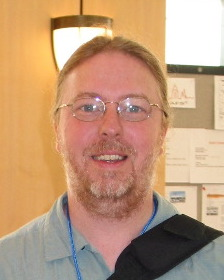
\includegraphics[width=\linewidth]{mugs/matt.jpg}

      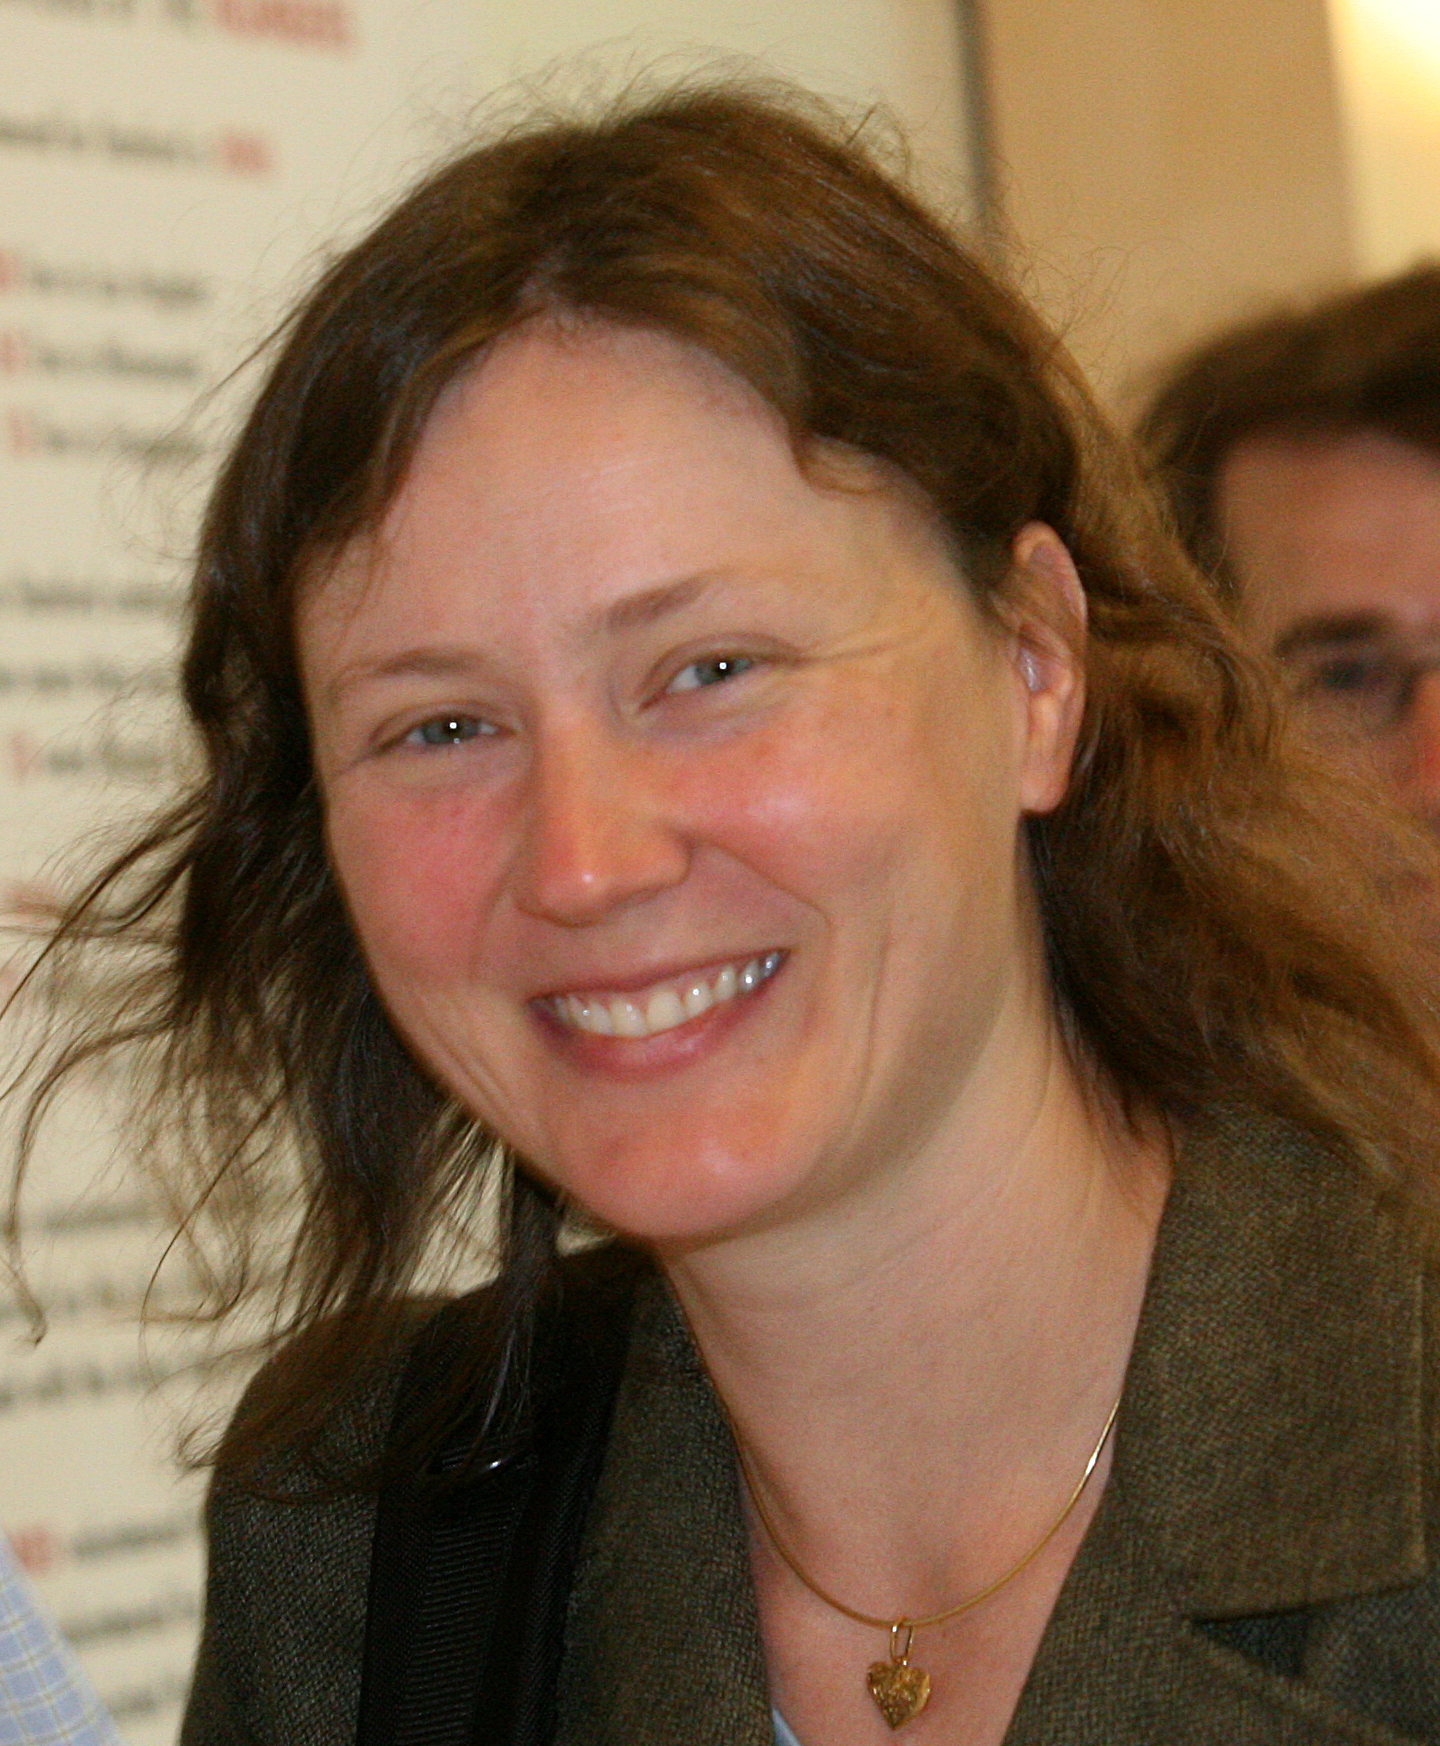
\includegraphics[width=\linewidth]{mugs/shelly.jpg}

      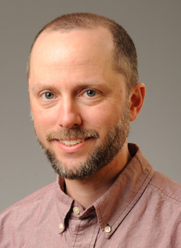
\includegraphics[width=\linewidth]{mugs/scott.jpg}

      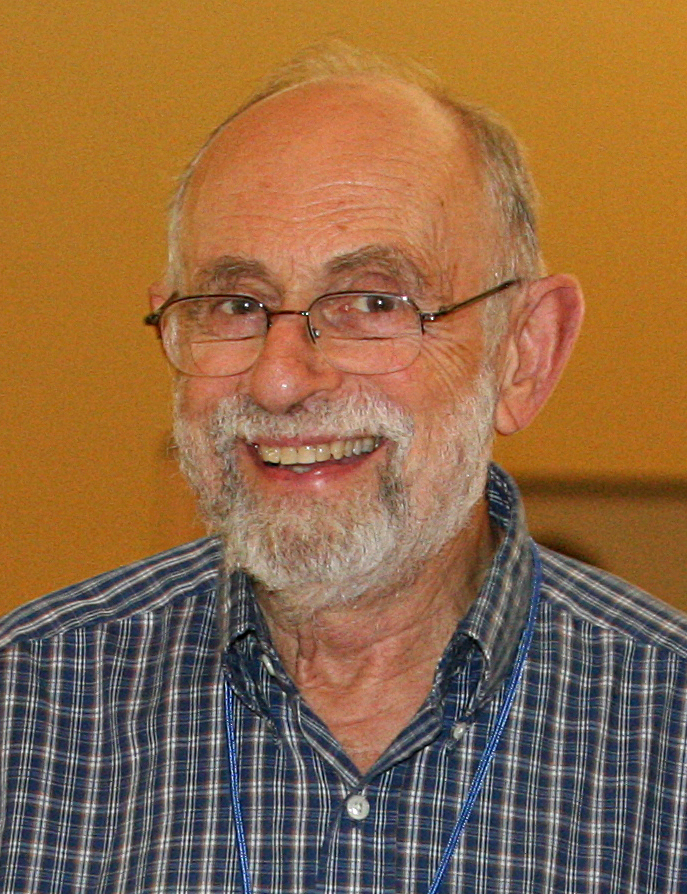
\includegraphics[width=\linewidth]{mugs/ed.jpg}

      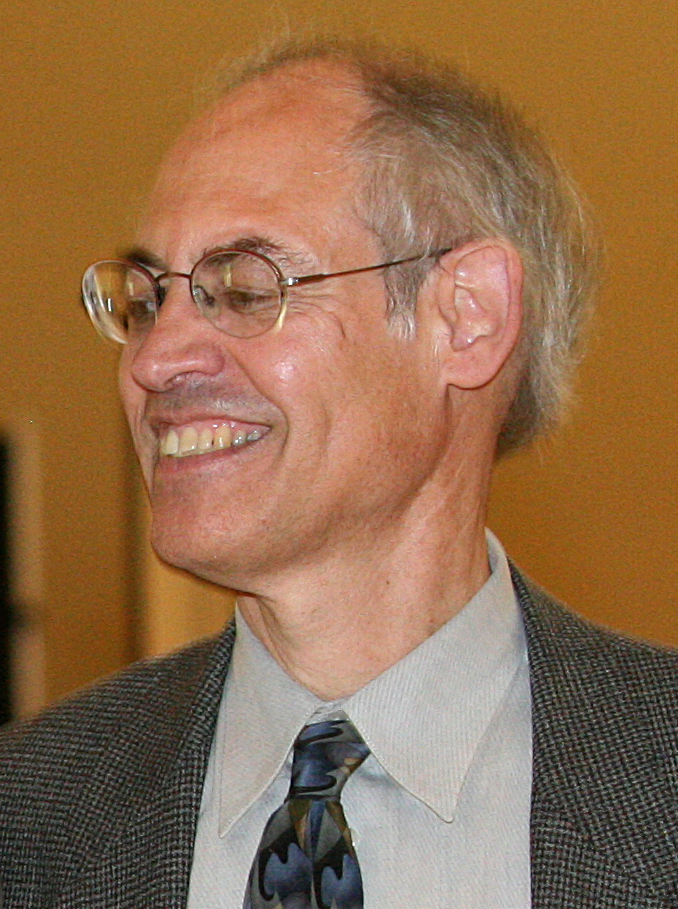
\includegraphics[width=\linewidth]{mugs/john.jpg}
    \end{column}
  \end{columns}
\end{frame}

\section{Why we measure XAS}

\begin{frame}
  \frametitle{The measurement goals of an XAS experiment}

  Somehow the wiggles in the XAS data tell us something about the
  atomic and electronic structure of the material measured.

  \medskip

  \begin{columns}
    \begin{column}{0.125\linewidth}
      ~
    \end{column}
    \begin{column}{0.45\linewidth}
      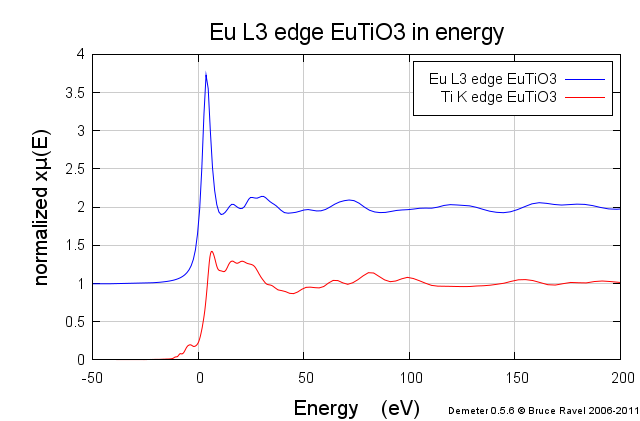
\includegraphics[width=\linewidth]{images/eto_mu.png}
    \end{column}
    \begin{column}{0.30\linewidth}
      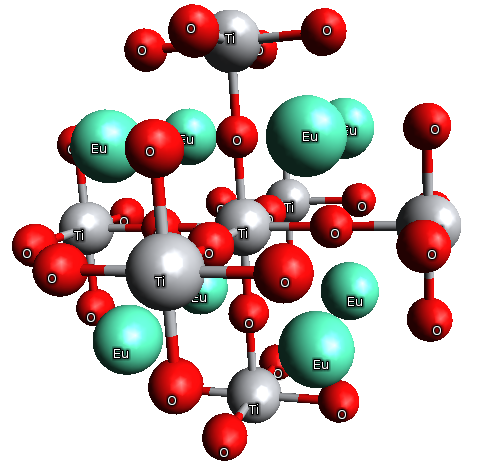
\includegraphics[width=\linewidth]{../ATEA/mds/eto.png}
    \end{column}
    \begin{column}{0.125\linewidth}
      ~
    \end{column}
  \end{columns}

  \medskip

  \begin{description}
  \item[Valence] the charge state of the absorber
  \item[Species] what kinds of atoms surround the absorber
  \item[Number] how many of those atoms there are
  \item[Distance] how far away they are
  \item[Disorder] how they are distributed due to thermal motion and
    structural disorder
  \end{description}
\end{frame}

\begin{frame}
  \frametitle{What can XAS be measured on}
  Well ... just about anything and with most elements of the periodic
  table

  \begin{columns}[T]
    \begin{column}{0.5\linewidth}
      \begin{exampleblock}{No assumption of symmetry or periodicity}
        \begin{itemize}
        \item Crystals
        \item Liquids or amorphous/highly disordered solids
        \item Mixed phases
        \item Thin films and engineered materials
        \item Surface sorbed species
        \item Organic and organometallic species
        \item Quasicrystals
        \item and on and on
        \end{itemize}
      \end{exampleblock}
    \end{column}
    \begin{column}{0.5\linewidth}
      \begin{alertblock}{Beamline choice and
          sample preparation matter}
        \begin{itemize}
        \item The beamline covers the absorber edge energy
        \item Sample is homogeneous
        \item Sample is not too thick, not too thin
        \item Sample is properly contained
        \end{itemize}
      \end{alertblock}
    \end{column}
  \end{columns}

\end{frame}

\begin{frame}
  \frametitle{Who uses XAS}
  Look to your left and right.  If you study catalysis, you may be
  sitting next to a biologist.  If you are a materials scientist, you
  might be sitting next to a geologist.

  \begin{block}{This fall,$^\ast$ just at my beamline NSLS X23A2, the users include}
    \begin{itemize}
    \item 2 groups from the microelectronics industry
    \item 2 groups of electrochemists
    \item a group working on fuel cell catalysts
    \item a group working on photocathode materials
    \item a group working on nuclear waste containment
    \item a group working on materials for nuclear reactor vessels
    \end{itemize}
  \end{block}

  to say nothing of the biologists, enironmental scientists,
  geologists, and chemical scientists visiting the other beamlines at
  NSLS at the same time.

  \begin{bottomnote}[0.5][20]
    $^\ast$September-December 2011
  \end{bottomnote}
\end{frame}

\section{How we measure XAS}

\begin{frame}
  \frametitle{Sometimes XAS is easy...}
  \begin{columns}
    \begin{column}{0.60\linewidth}
      Here we have a \textit{single scan} of the Ge K edge of a 50\,nm
      film of Ge/Sb alloy on silica measured at glancing angle on a
      beamline (NSLS X23A2) without focusing optics and using a
      Si(311) crystal.
    \end{column}
    \begin{column}{0.36\linewidth}
      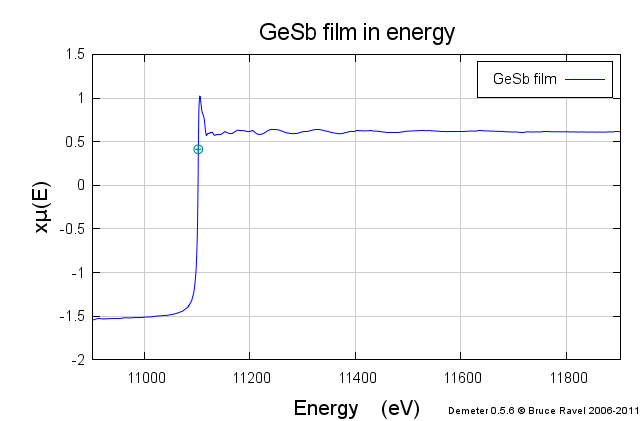
\includegraphics[width=\linewidth]{images/gesb_mu.png}

      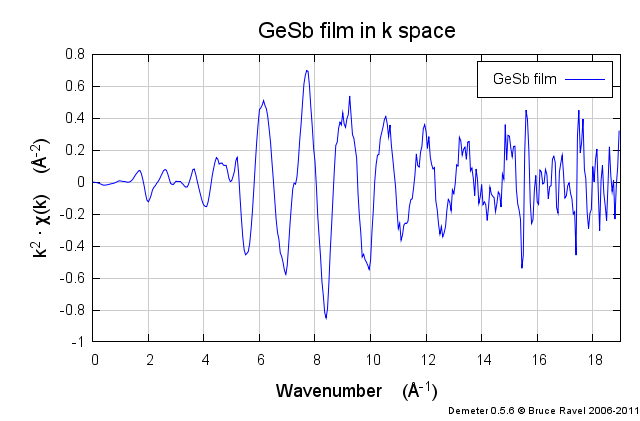
\includegraphics[width=\linewidth]{images/gesb_chik.png}      

      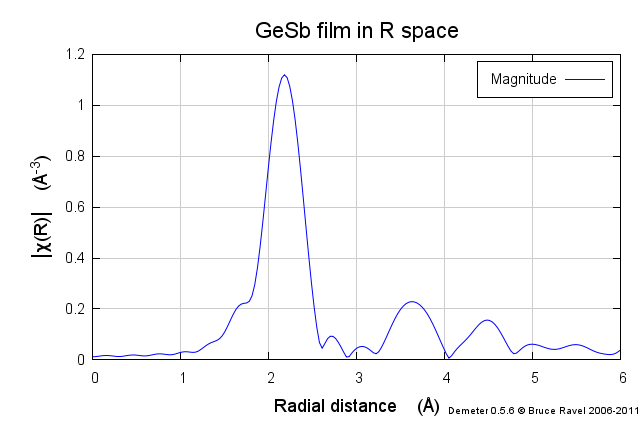
\includegraphics[width=\linewidth]{images/gesb_chir.png}
    \end{column}
  \end{columns}
  \begin{bottomnote}[0.4][19.0]
    These data are courtesy of Joseph Washington and Eric
    Joseph (IBM Research)
  \end{bottomnote}
\end{frame}

\begin{frame}
  \frametitle{Sometimes XAS is hard...}
  \begin{columns}
    \begin{column}{0.60\linewidth}
      Here are 42 scans taken over the course of 22 hours at APS 20BM
      (one of the top XAS beamlines in North America) on a sample with
      3\,mM Hg bound to an engineered DNA complex.

      \medskip

      Each scan is quite noisy, but the central limit theorem
      \textit{always} works.  We were able to use the resulting
      $\tilde\chi(R)$ data to good effect.
    \end{column}
    \begin{column}{0.36\linewidth}
      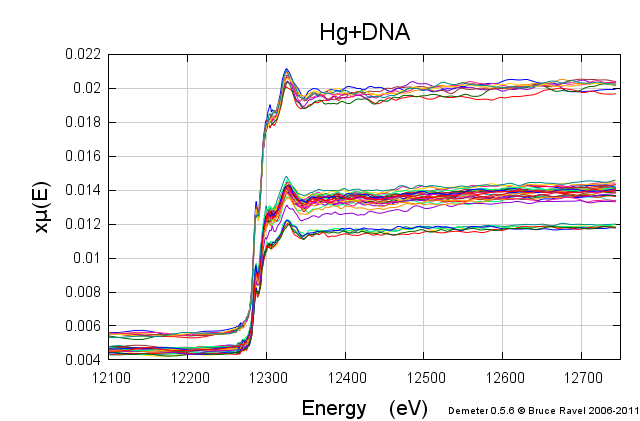
\includegraphics[width=\linewidth]{images/hg_mu_stack.png}

      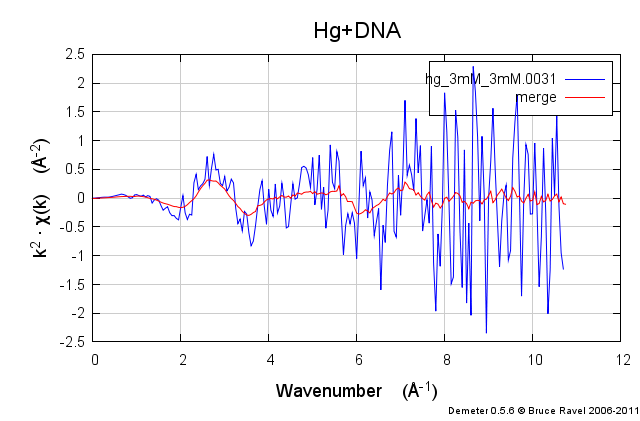
\includegraphics[width=\linewidth]{images/hg_chik.png}      

      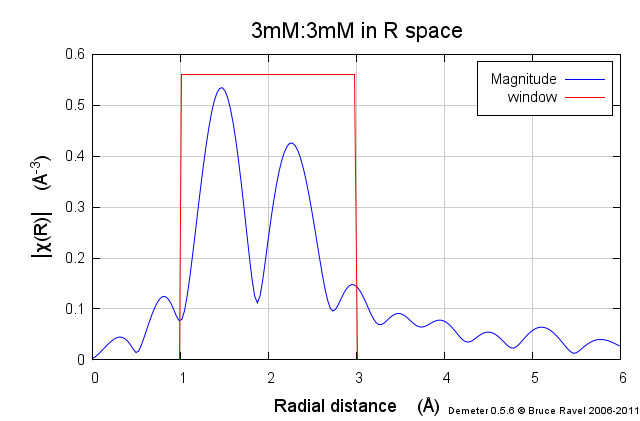
\includegraphics[width=\linewidth]{../ATEA/info/hgdna_chir.png}
    \end{column}
  \end{columns}
  \begin{bottomnote}[0.4][18.0]
    B.\ Ravel, et al., \textit{EXAFS studies of catalytic DNA sensors
      for mercury contamination of water}, Radiation Physics and
    Chemistry \textbf{78}:10 (2009) pp\ S75-S79.
    \doiref{10.1016/j.radphyschem.2009.05.024}[LightBlue4]
  \end{bottomnote}
\end{frame}

\begin{frame}
  \frametitle{In any case...}
  Regardless of how easy or difficult an experiment is, we have to
  know how to
  \begin{itemize}
  \item<1-> Evaluate the statistical quality of our data
  \item<2-> Recognize both statistical and systematic errors in our data
    and understand how to address each kind of error
  \item<3-> Know when to stop measuring a sample -- I mean this both in
    the sense of knowing how far above the edge to measure and knowing
    how many repetitions to measure
  \item<4-> Know how to process our data for further analysis
  \end{itemize}
\end{frame}

\begin{frame}
  \frametitle{Sometimes we do elaborate experiments}
  \begin{block}{}
    New technologies and modern, 3$^{\mathrm{rd}}$ generation
    synchrotrons offer intriguing new experimental possibilties.
  \end{block}

  \bigskip

  \begin{alertblock}{}
    In each case, one of the results of these elaborate experiments is
    an XAS spectrum.
  \end{alertblock}
\end{frame}

\begin{frame}
  \frametitle{Imaging and $\mu$XAS}
  \begin{columns}[T]
    \begin{column}{0.4\linewidth}
      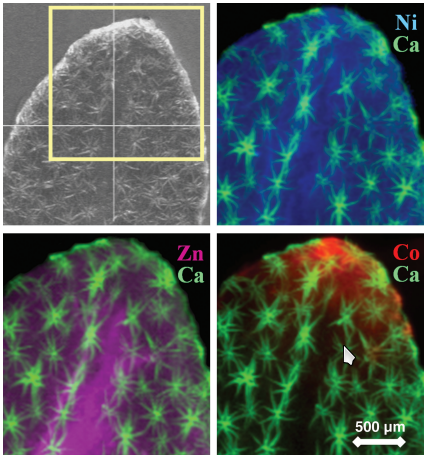
\includegraphics[width=\linewidth]{images/xrfmap.png}
    \end{column}
    \begin{column}{0.6\linewidth}
      Here is an extraordinary XRF map of a metal hyperaccumulating
      plant that also forms star-shaped, inorganic nodules on its
      leaves.  
      
      \smallskip

      \begin{overlayarea}{\linewidth}{9ex}
        \only<2>{\alert{While the image is itself a great result, we
            end up measuring XAS spectra with the microbeam.}}
      \end{overlayarea}

      \begin{overlayarea}{\linewidth}{9ex}
        \begin{center}
          \includegraphics<2>[width=0.8\linewidth]{images/xrfxas.png}
        \end{center}
      \end{overlayarea}

    \end{column}
  \end{columns}
  \begin{bottomnote}[0.6][19]
    R.\ Tappero, et al., \textit{Hyperaccumulator Alyssum murale
      relies on a different metal storage mechanism for cobalt than
      for nickel}, New Phytologist \textbf{175}:4
    (2007) pp\ 641-654
    \doiref{10.1111/j.1469-8137.2007.02134.x}[LightBlue4]
  \end{bottomnote}
\end{frame}

\begin{frame}
  \frametitle{Time-resolved XAS and mountains of data}

  \begin{columns}[T]
    \begin{column}{0.55\linewidth}
      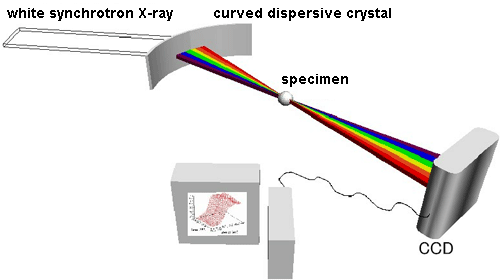
\includegraphics[width=0.8\linewidth]{images/ede.png}
    \end{column}
    \begin{column}{0.42\linewidth}
      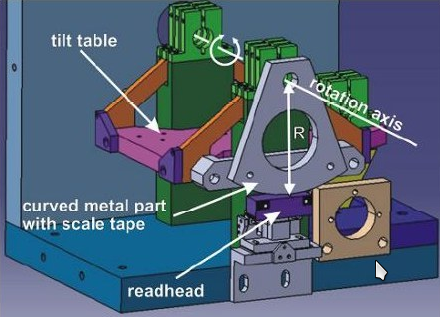
\includegraphics[width=0.8\linewidth]{images/qxas_mono.png}
    \end{column}
  \end{columns}

  \begin{columns}
    \begin{column}{0.5\linewidth}
      \begin{overlayarea}{\linewidth}{24ex}
        Energy dispersive XAS and quick-XAS are two ways of doing
        time-resolved XAS with 10\,ms to 10\,s time resolution.  Both
        approaches require specially- equipped beamlines and both
        focus on the dynamics of the system. \only<2>{\alert{At then
            end of the day, these are XAS spectra.}}
      \end{overlayarea}
    \end{column}
    \begin{column}{0.5\linewidth}
      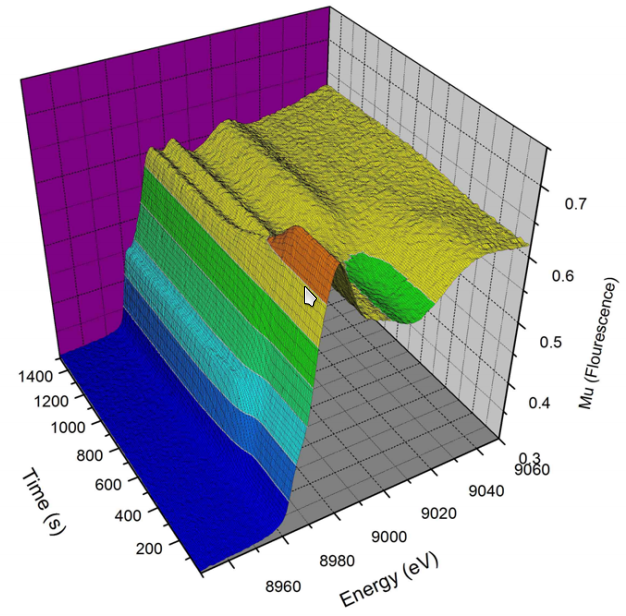
\includegraphics[width=0.8\linewidth]{images/qxas.png}
    \end{column}
  \end{columns}

  \begin{bottomnote}[0.7][19.5]
    Data from W.A.\ Caliebe et al., \textit{HASYLAB Annual Report}
    (2006) pp.\ 283-284; EDE schematic from SPring-8 press release, 30
    April, 2009; QXAS schematic from SLS SuperXAS beamline webpage.
  \end{bottomnote}
\end{frame}

\begin{frame}
  \frametitle{Diffraction Anomalous Fine Structure}

  With coordinated motion between monochromator and goniometer, DAFS
  measures the height of a diffraction peak with respect to energy
  through the resonant energy of an atom in the crystal.
  \begin{columns}[T]
    \begin{column}{0.5\linewidth}
      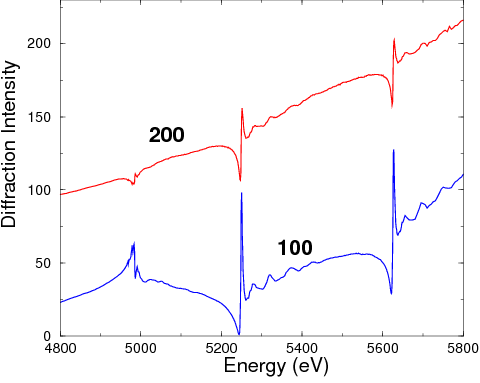
\includegraphics[width=0.85\linewidth]{images/dafs.png}
    \end{column}
    \begin{column}{0.5\linewidth}
      \includegraphics<2>[width=0.8\linewidth]{images/dafschik.png}      
    \end{column}
  \end{columns}
  \begin{overlayarea}{\linewidth}{6ex}
    \only<2>{\alert{In the end, we extract a site-specific $\chi(k)$
        function which is analyzed like normal EXAFS.}}
  \end{overlayarea}

  \begin{bottomnote}[0.6][19.5]
    B.\ Ravel et al., \textit{X-ray-absorption edge separation using
      diffraction anomalous fine structure}, Phys.\ Rev.\ B \textbf{60}
    (1999) pp\ 778-785.
    \doiref{10.1103/PhysRevB.60.778}[LightBlue4]
  \end{bottomnote}
\end{frame}

\begin{frame}
  \frametitle{Non-resonant Inelastic X-ray Scattering}

  \small
  Here is NIXS data from a non-resonant inelastic scattering data on
  CaZrTi$_2$O$_7$ from 20ID at APS.
  \begin{columns}[T]
    \begin{column}{0.42\linewidth}
      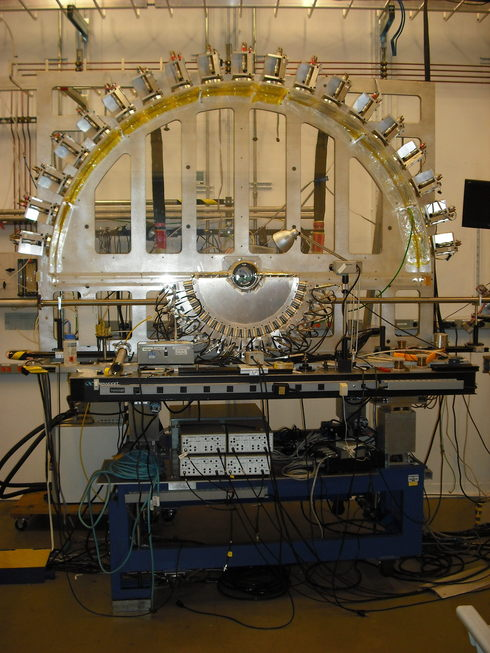
\includegraphics[width=\linewidth]{images/lerix_sm.jpg}
    \end{column}
    \begin{column}{0.6\linewidth}
      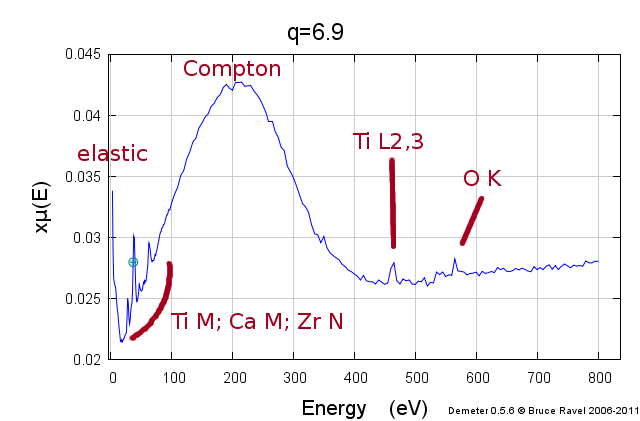
\includegraphics[width=0.7\linewidth]{images/nixs.png}

      \includegraphics<2>[width=0.7\linewidth]{images/TiL23.png}
    \end{column}
  \end{columns}

  \begin{overlayarea}{\linewidth}{2ex}
    \only<2>{\alert{Again, a XANES spectrum comes from this elaborate
        experiment.}}
  \end{overlayarea}
  \begin{bottomnote}[0.7][20]
    Lerix-I instrument: G.\ Seidler et al.; Data:
    D.\ Reid, N.C.\ Hyatt, B.\ Ravel, to be published in PRB
  \end{bottomnote}
\end{frame}


\section{How we use XAS}

\begin{frame}
  \frametitle{Some vocabulary}
  Words commonly used to describe specific parts of the XANES spectrum.

  \begin{columns}[T]
    \begin{column}{0.5\linewidth}
      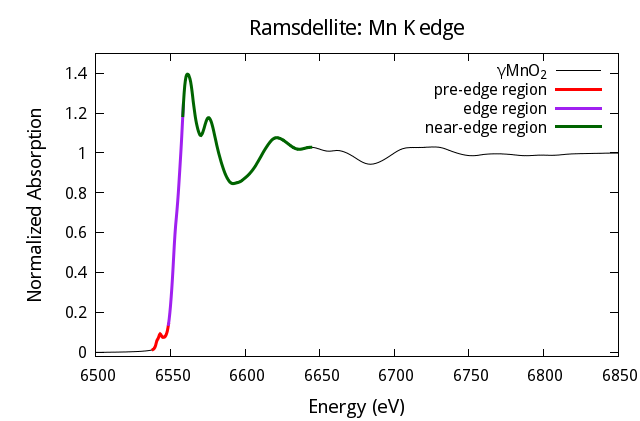
\includegraphics[width=\linewidth]{../i2x/images/rams/ramsdellite.png}

      \small

      \begin{description}[edge]
      \item[{\color{red}pre-edge}] Small (possibly large, certainly
        meaningful!) features between the Fermi energy and the
        threshold
      \item[{\color{DarkOrchid2}edge}] The main rising part of XAS spectrum
      \item[{\color{Green4}near-edge}] Characteristic features above the edge
      \end{description}
    \end{column}    
    \begin{column}{0.5\linewidth}
      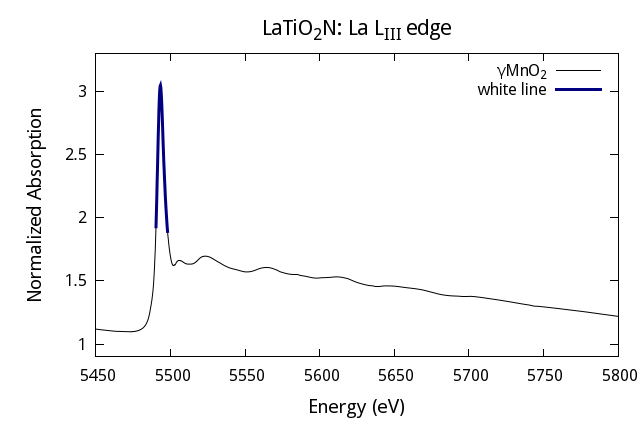
\includegraphics[width=\linewidth]{../i2x/images/ltno/ltno.png}

      \begin{description}[wh]
      \item[{\color{Blue3}white line}] Large, prominent peak just
        above the edge, particularly in L or M edge spectra
      \end{description}

      \bigskip

      \begin{block}{}
        The EXAFS, then, is the data beyond the
        {\color{Green4}near-edge}.
      \end{block}
    \end{column}    
  \end{columns}
\end{frame}

\begin{frame}
  \frametitle{Fingerprinting}
  The simplest way of using XAS is to simply identify chemical species
  in a sample of unknown composition.

  \begin{columns}
    \begin{column}{0.5\linewidth}
      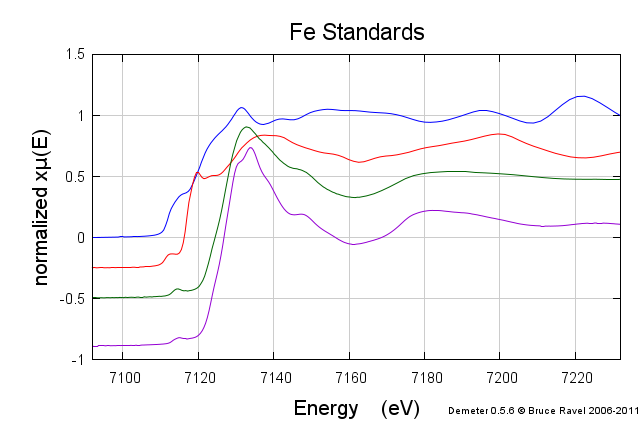
\includegraphics[width=\linewidth]{images/fe_stan.png}
    \end{column}
    \begin{column}{0.25\linewidth}
      \begin{enumerate}
      \item \only<1|handout:0>{Ferrihydrite?}\only<2|handout:1>{\color{Green4}Ferrihydrite}
      \item \only<1|handout:0>{Iron pyrite?}\only<2|handout:1>{\color{Red3}Iron pyrite}
      \item \only<1|handout:0>{Iron metal?}\only<2|handout:1>{\color{Blue4}Iron metal}
      \item \only<1|handout:0>{Hematite?}\only<2|handout:1>{\color{Purple4}Hematite}
      \end{enumerate}
    \end{column}
    \begin{column}{0.15\linewidth}
    \end{column}
  \end{columns}
  
  \bigskip

  \begin{overlayarea}{\linewidth}{4ex}
    \only<2|handout:1>{Compare the signal from your \textit{( dirt /
        catalyst / paint chip / animal tissue / whatever )} with
      the standards to identify the dominant species.}
  \end{overlayarea}
  \only<handout>{
    \begin{bottomnote}[0.7][19.5]
      (For the color-blind: The spectra, top-to-bottom, are metal,
      pyrite, ferrihydrite, and hematite.)
    \end{bottomnote}
  }
\end{frame}

\begin{frame}
  \frametitle{XANES Interpretation}
  Fingerprinting, though useful, is purely qualitative.

  \bigskip

  There are a variety of quantitive tools available for interpreting
  XANES data.
  \begin{enumerate}
  \item Positioning
  \item Peak fitting
  \item Linear combination fitting
  \item Principle components analysis
  \item Application of theory
  \end{enumerate}
\end{frame}

\begin{frame}
  \frametitle{XANES: Positioning}
  \begin{columns}[T]
    \begin{column}{0.5\linewidth}
      \small%
      U$^{6+}$ is partially reduced by \textit{G. sulfurreducens}
      under a variety of conditions.  By measuring the edge positions
      and comparing to U$^{6+}$ and U$^{4+}$ standards,
      the amount of reduction is quatified between 24\% and 88\%.

      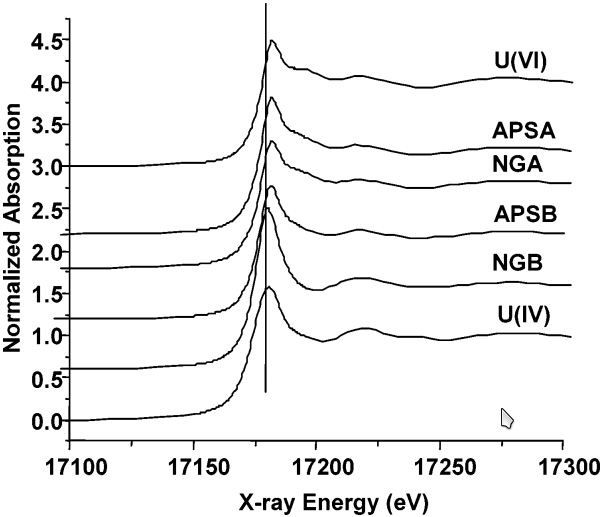
\includegraphics[width=0.8\linewidth]{images/u46.png}      
    \end{column}
    \begin{column}{0.5\linewidth}
      \small%
      Farges et al. showed that Ti clusters by valence when the
      position of the largest {\color{red}pre-edge} is plotted against
      peak position in energy.

      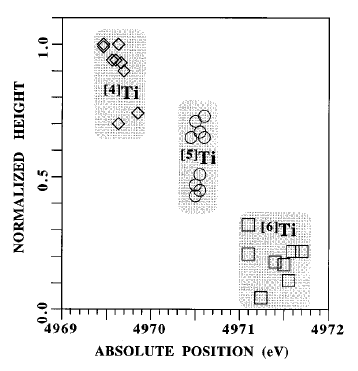
\includegraphics[width=0.8\linewidth]{../selfabs/images/farges.png}      
    \end{column}
  \end{columns}
  \begin{exampleblock}<2>{}
    \small%
    \qquad Either analysis requires careful attention to data processing.
  \end{exampleblock}
  \begin{bottomnote}[0.5][19]
    B.H.\ Jeon et el., \textit{Microbial Reduction of U(VI) at the
      Solid-Water Interface}, Environ. Sci. Technol. \textbf{38}(21)
    pp.~5649-5655. (2004), \doiref{10.1021/es0496120}[LightBlue4]
  \end{bottomnote}
  \begin{textblock*}{0.4\linewidth}(0.6\linewidth,19\TPVertModule)
    \tiny%
    \begin{color}{bngray}
      F.~Farges, G.E.~Brown, Jr., and J.J.~Rehr, PRB \textbf{56}:4,
      (1997) p.\ 1809.
    \end{color}
    \doiref{10.1103/PhysRevB.56.1809}[LightBlue4]
  \end{textblock*}

\end{frame}

\begin{frame}
  \frametitle{XANES: Peak fiting}
  \begin{columns}
    \begin{column}{0.5\linewidth}
      Peak fitting presumes that the XANES data can be explained as a
      sum of simple line shapes -- usually a combination of
      \begin{itemize}
      \item arctangent (for the edge step)
      \item Gaussian
      \item Lorentzian
      \item Voight or pseudo-Voight
      \end{itemize}
    \end{column}
    \begin{column}{0.5\linewidth}
      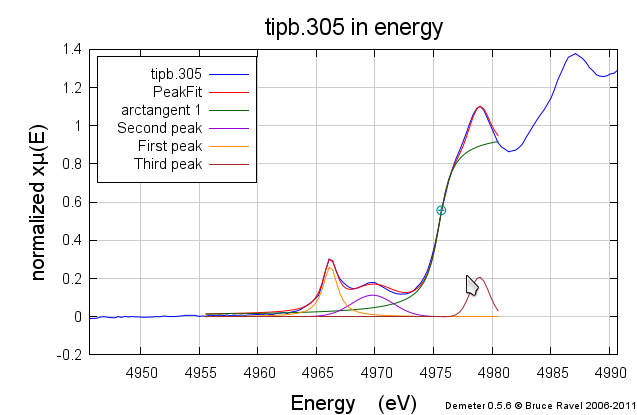
\includegraphics[width=\linewidth]{images/peakfit.png}
    \end{column}
  \end{columns}

  \bigskip

  \begin{block}{The shortcoming of peak fitting}
    It is difficult in general to ascribe physical meaning to the
    lineshapes.  Peak fitting is, therefore, best used to quantify
    changes in a related ensemble of data.
  \end{block}
\end{frame}

\begin{frame}
  \frametitle{XANES: Linear Combination Fitting}
  In this example, XAS is measured as a function of time as a gold
  chloride is reduced to metallic gold in the presence of sulfurous
  biomass.  At an intermediate time step, the spectrum is understood
  as a linear combination of the initial state
  ({\color{Green4}Au$^{3+}$Cl}), the final state ({\color{Purple4}Au
    metal}), and an intermediate state ({\color{Orange2}some Au$^{1+}$
    sulfide species}).
  \begin{columns}
    \begin{column}{0.5\linewidth}
      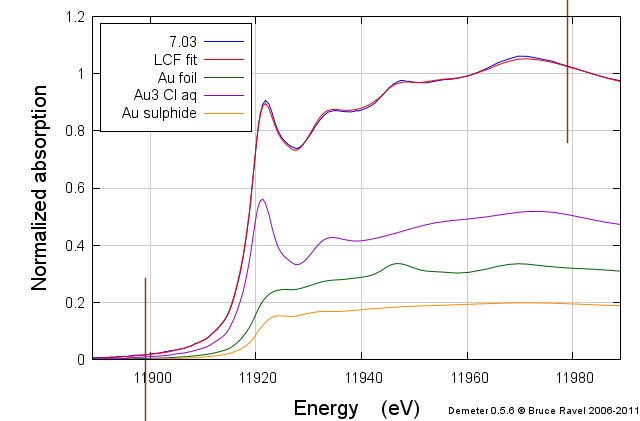
\includegraphics[width=\linewidth]{aucl/aucl_lcf.png}
    \end{column}
    \begin{column}{0.5\linewidth}
      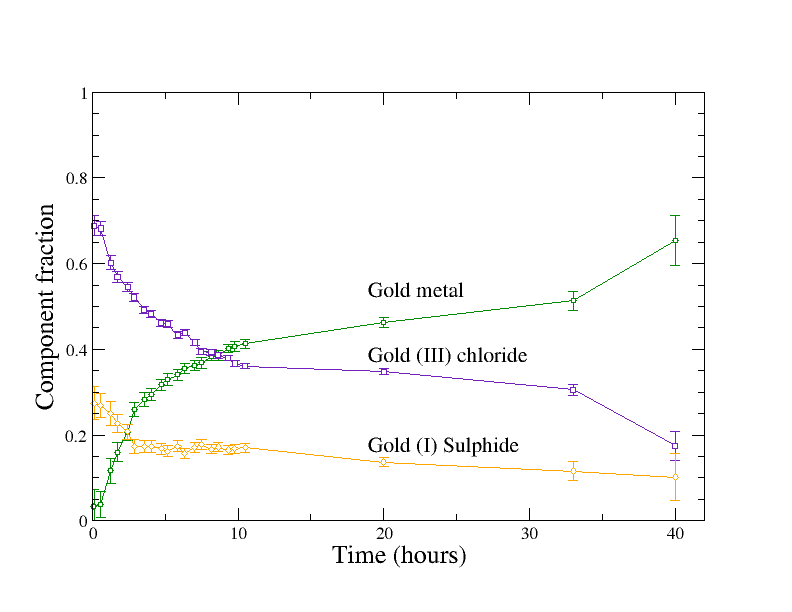
\includegraphics[width=\linewidth]{aucl/aucl_results.png}
    \end{column}
  \end{columns}
  \begin{flushright}
    \scriptsize (There will be an entire lecture on this topic tomorrow.)
  \end{flushright}
  \begin{bottomnote}[0.5][18.75]
    M. Lengke et el., \textit{Mechanisms of Gold Bioaccumulation by
      Filamentous Cyanobacteria from Gold(III)-Chloride Complex},
    Environ. Sci. Technol. \textbf{40}(20) p.~6304-6309. (2006),
    \doiref{10.1021/es061040r}[LightBlue4]
  \end{bottomnote}
\end{frame}

\begin{frame}
  \frametitle{XANES: Principle Components Analysis}
  \small%
  PCA is a bit of linear algebra which breaks down an ensemble of
  related data into abstract components.
  \begin{columns}[T]
    \begin{column}{0.33\linewidth}
      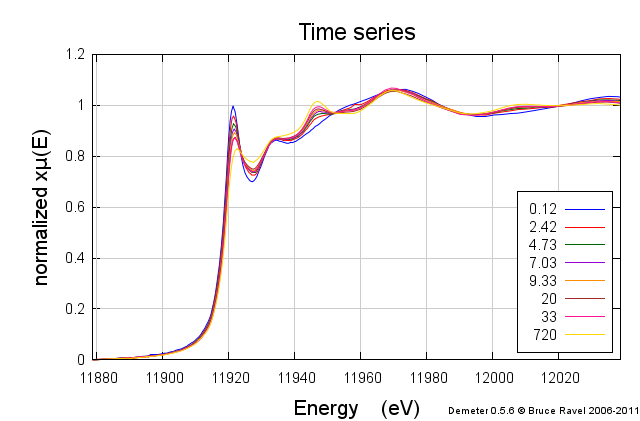
\includegraphics[width=\linewidth]{images/aucyano_time_series.png}
    \end{column}
    \begin{column}{0.33\linewidth}
      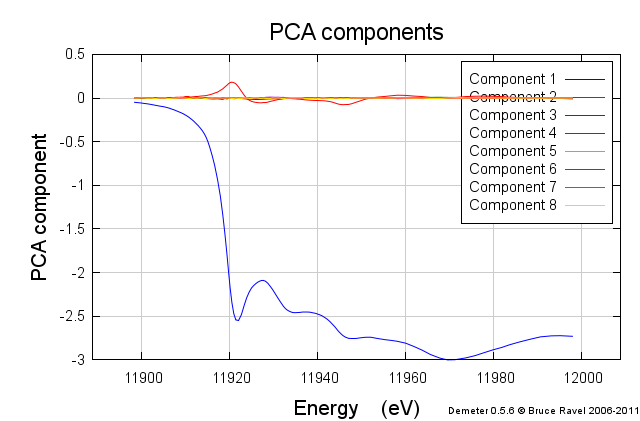
\includegraphics[width=\linewidth]{images/pca_all.png}      
    \end{column}
    \begin{column}{0.33\linewidth}
      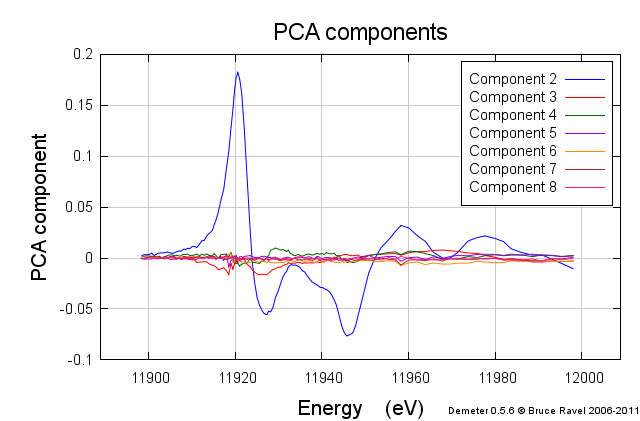
\includegraphics[width=\linewidth]{images/pca_2-8.png}            
    \end{column}
  \end{columns}

  \medskip

  The components can then be used to try to construct a standard as a
  test to see whether that standard is present in the ensemble.

  \medskip

  \begin{columns}
    \begin{column}{0.33\linewidth}
      The number of species represented in the ensemble is related to
      the number of statistically significant components.
    \end{column}
    \begin{column}{0.33\linewidth}
      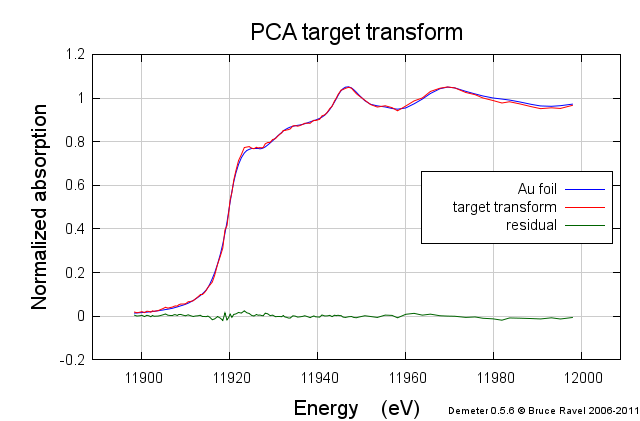
\includegraphics[width=\linewidth]{images/pca_tt_in.png}
    \end{column}
    \begin{column}{0.33\linewidth}
      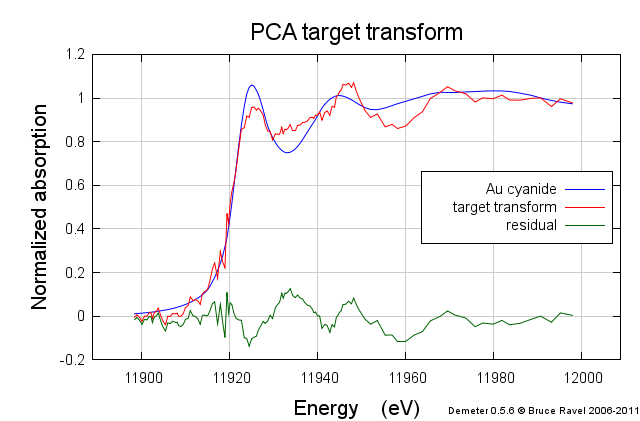
\includegraphics[width=\linewidth]{images/pca_tt_out.png}
    \end{column}
  \end{columns}
  \begin{bottomnote}[0.48][19]
    The data in the upper left are from M. Lengke et el.,
    Environ. Sci. Technol. \textbf{40}(20) p.~6304-6309. (2006),
    \doiref{10.1021/es061040r}[LightBlue4].  That paper did not
    include any PCA analysis.
  \end{bottomnote}
\end{frame}

\begin{frame}
  \frametitle{XANES: Theory}
  \begin{columns}
    \begin{column}{0.5\linewidth}
      \begin{center}
        Forward simulation with \textsc{feff}9
      \end{center}
      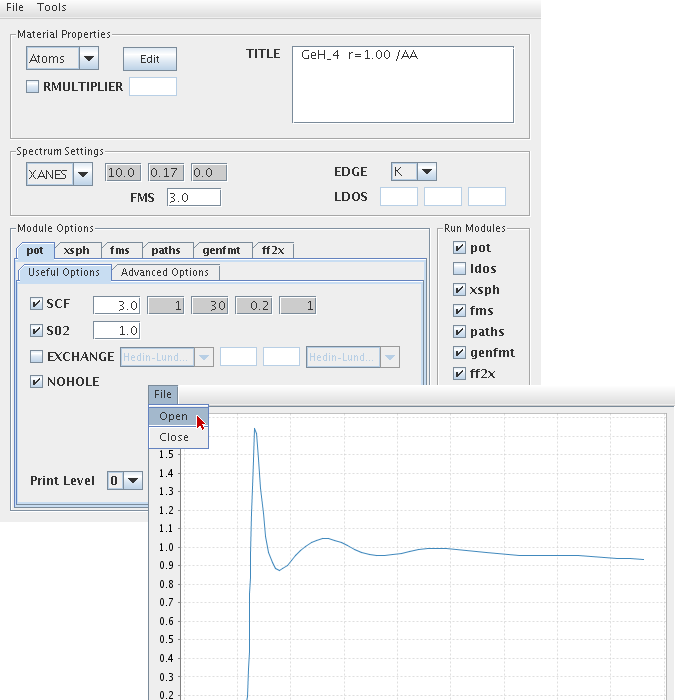
\includegraphics[width=\linewidth]{images/jfeff.png}
    \end{column}
    \begin{column}{0.5\linewidth}
      \begin{itemize}
      \item Fitting of XANES spectra is not built into \textsc{feff},
        but other options exist
      \item \textsc{mxan} by Benfatto and Della Longa allows variation
        of structural parameters to refine a full multiple scattering
        calculation against measured data
      \item \textsc{FitIt} by Smolentsev and Soldatov fits measured
        data by pre-computing spectra on a multidimensional grid of
        caluclated spectra and interpolating to best fit the data.  It
        can use either \textsc{feff} or Joly's \textsc{fdmnes}
      \end{itemize}

    \end{column}
  \end{columns}

  \begin{bottomnote}[0.7][19]
    \href{http://leonardo.phys.washington.edu/feff/}
    {\color{LightBlue4}{\ComputerMouse~}Feff homepage: \texttt{http://leonardo.phys.washington.edu/feff/}}%
    \\
    \href{http://www.esrf.eu/computing/scientific/MXAN/index.html}
    {\color{LightBlue4}{\ComputerMouse~}MXAN homepage: \texttt{http://www.esrf.eu/computing/scientific/MXAN/index.html}}%
    \\
    \href{http://www.nano.sfedu.ru/index.html} 
    {\color{LightBlue4}{\ComputerMouse~}FitIt homepage: \texttt{http://www.nano.sfedu.ru/index.html}}
  \end{bottomnote}
\end{frame}


\begin{frame}
  \frametitle{EXAFS analysis can be simple...}

  \begin{center}
    Here is a quick first shell fit to the Fe K edge of lepidocrocite,
    $\gamma$-FeO(OH).
  \end{center}
  \begin{columns}
    \begin{column}{0.45\linewidth}
      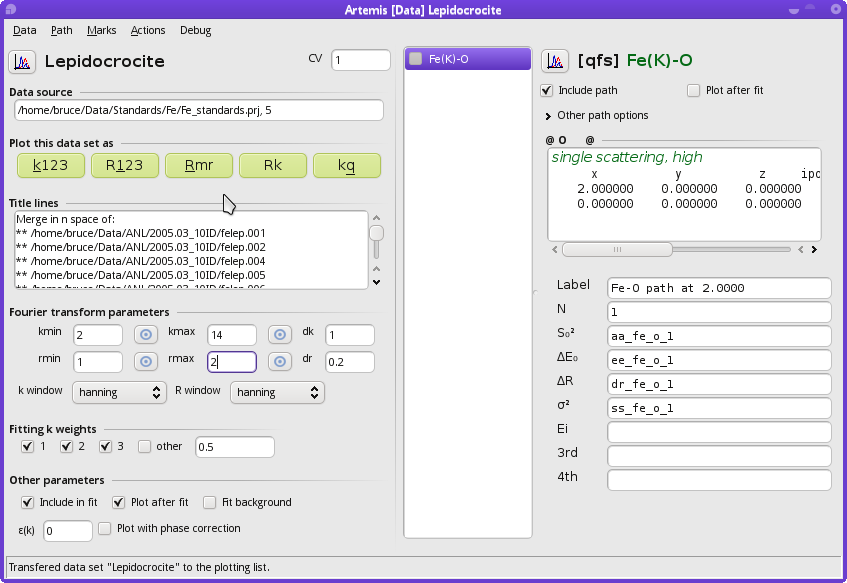
\includegraphics[width=\linewidth]{images/qfs.png}
    \end{column}
    \begin{column}{0.5\linewidth}
      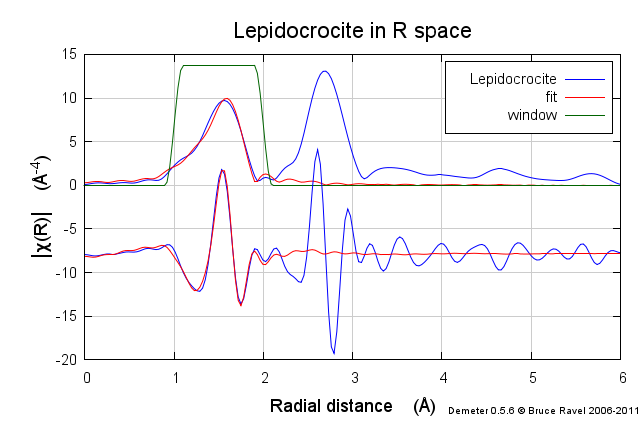
\includegraphics[width=\linewidth]{images/qfs_fit.png}      
    \end{column}
  \end{columns}
  \begin{center}
    Using \textsc{artemis} and a simple first shell fitting model, it
    takes under a minute to fill in all the boxes and to get a fit of
    this quality, providing a first stab at near-neighbor coordination
    and distance.
  \end{center}
  \begin{block}{}
    \begin{center}
      Fit: $\mathrm{N=4}.6\pm0.3$, $\mathrm{R}=2.01\pm0.01$, $\sigma^2=0.00586\pm0.00088$\\
      Crystal structure: $\mathrm{N=5}$, $\bar{\mathrm{R}}=2.05$, $\mathrm{C}_2=0.00679$
    \end{center}
  \end{block}

\end{frame}

\begin{frame}
  \frametitle{EXAFS analysis can be sophisticated...}
  \begin{block}{}
    \begin{center}
      Well ... this is the point of this course!
    \end{center}
  \end{block}

  You will learn how to:
  \begin{enumerate}
  \item Use one or more \textsc{feff} to fit your data
  \item Build interesting contraints between and restraints on your
    fitting parameters
  \item Do multiple data set fitting
  \item Do multiple k-weight fitting
  \item Evaluate the statistical quality of your fits
  \item Present your fitting results defensibly in journal articles
  \end{enumerate}
\end{frame}

\begin{frame}
  \frametitle{EXAFS analysis can be quite elaborate...}
  \begin{columns}[T]
    \begin{column}{0.2\linewidth}
      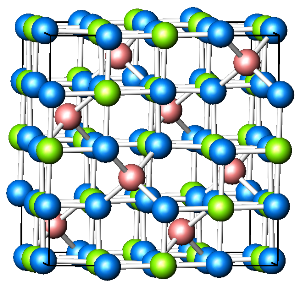
\includegraphics[width=\linewidth]{images/ferrite.png}
      \begin{center}
        {\color{Blue3}Oxygen}\\{\color{Green3}Octahedral site}
        \\{\color{Red3}Tetrahedral site}
      \end{center}
    \end{column}
    \begin{column}{0.3\linewidth}
      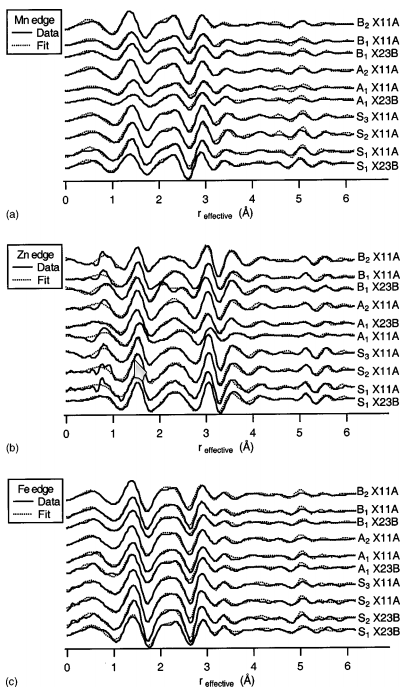
\includegraphics[width=\linewidth]{images/ferrite_fits.png}
    \end{column}
    \begin{column}{0.5\linewidth}
      \begin{itemize}
      \item Manganese zinc ferrite nanoparticles
      \item Each element can occupy each either metal site
      \item Oxygen vacancies can exist
      \item Data collected at 3 edges and on various sample
        preparations
      \item Scott created a fitting model using all the data
        simultaneously and considering occupancies of each metal on
        each site, oxygen vacancy, and nanoparticle undercoordination
      \end{itemize}
    \end{column}
  \end{columns}
  \begin{bottomnote}[0.7][18.75]
    S.\ Calvin et el., \textit{Multiedge refinement of extended
      x-ray-absorption fine structure of manganese zinc ferrite
      nanoparticles}, Phys. Rev. B \textbf{66}(22) p.~224405. (2002),
    \doiref{10.1103/PhysRevB.66.224405}[LightBlue4]\\
    Ferrite image from
    \href{http://wikis.lib.ncsu.edu/index.php/Image:Size21.png}
    {\color{LightBlue4}{\ComputerMouse~}\texttt{http://wikis.lib.ncsu.edu/index.php/Image:Size21.png}}
  \end{bottomnote}
\end{frame}

\section{How we understand XAS}

\begin{frame}
  \frametitle<1| handout:1>{A simple picture of X-ray absorption} 
  \frametitle<2| handout:2>{X-ray absorption in condensed matter}

  \begin{overlayarea}{\linewidth}{6ex}
    \only<1| handout:1>{An incident x-ray of energy $E$ is absorbed,
      destroying a core electron of binding energy $E_0$ and emitting
      a photo-electron with kinetic energy $(E-E_0)$. The core state
      is eventually filled, ejecting a fluorescent x-ray or an Auger
      electron.  }%
    \only<2| handout:2>{The ejected photo-electron can scatter from
      neighboring atoms. $R$ has some relationship to $\lambda$ and
      there is a phase shift associated with the scattering event.
      Thus the outgoing and scattered waves interfere.  }%
  \end{overlayarea}

  \vskip 20pt

  \begin{columns}[T]
    \begin{column}{0.5\linewidth}
      \only<1| handout:1>{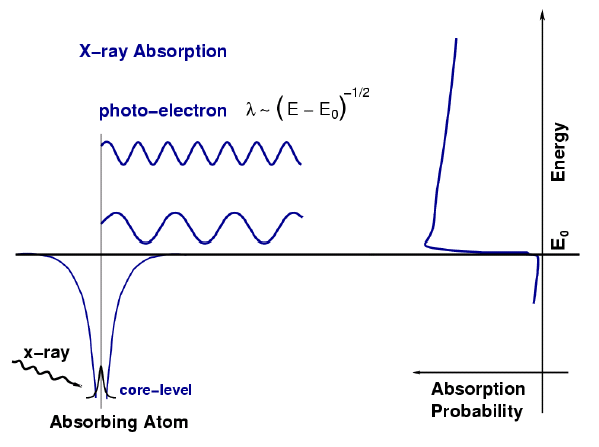
\includegraphics[width=\linewidth]{bare_atom.png}}
      \only<2| handout:2>{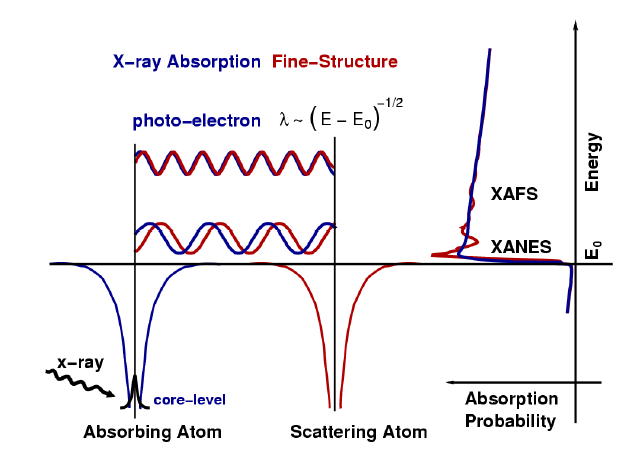
\includegraphics[width=\linewidth]{with_scattering.png}}
    \end{column}
    \begin{column}{0.5\linewidth}
      \begin{center}
        \only<1| handout:1>{
          An empty final state is required.\\
          {\alert{No available state, \\
              no absorption!}}\\
          When the incident x-ray energy is larger than the binding
          energy, there is a sharp increase in absorption.
        }
        \only<2| handout:2>{
          The scattering of the photo-electron wave function interferes
          with itself.\\[4ex]
          $\mu(E)$ depends on the density of states with energy
          $(E-E_0)$ at the absorbing atom.
        }
      \end{center}
    \end{column}
  \end{columns}

  \vskip 20pt

  \begin{overlayarea}{\linewidth}{3ex}
    \only<1| handout:1>{For an isolated atom, $\mu(E)$ has a sharp step at the
      core-level binding energy and is a smooth function of energy
      above the edge.}%
    \only<2| handout:2>{This interference \alert{at the absorbing atom} will vary
      with energy, causing the oscillations in $\mu(E)$.
    }%
  \end{overlayarea}
  \begin{bottomnote}[0.7][20] 
    Image from Matt Newville
  \end{bottomnote}
\end{frame}

\newcommand{\GMS}{\mathbb{G}}
\newcommand{\Gnot}{\mathsf{G^0}}
\newcommand{\tmat}{\mathsf{t}}
\newcommand{\boldr}{\boldsymbol{r}}

\begin{frame}[label=fgr]
  \frametitle{Computing X-ray Absorption from First Principles}
  \begin{columns}
    \begin{column}{0.75\linewidth}
      In XAS we measure the \alert{dipole mediated}$^\mathrm{[1]}$
      transition of an electron in a \alert{deep core}$^\mathrm{[2]}$
      state {\color{blue}$|i\rangle$} into an
      \alert{unoccupied}$^\mathrm{[3]}$ state
      {\color{Red4}$|f\rangle$}:

      \begin{columns}
        \begin{column}{0.15\linewidth}
          ~
        \end{column}
        \begin{column}{0.7\linewidth}
          \begin{block}{Fermi's Golden Rule}
            $\mu(E) \propto\> \sum\limits_f^{E_f>E_F}
            \big|{\color{Red4}\langle f|}
            {\color{blue}\hat{\epsilon}\cdot\mathbf{r}}
            {\color{blue}|i\rangle}\big|^2 \delta(E_f)$
          \end{block}
        \end{column}
        \begin{column}{0.15\linewidth}
          ~
        \end{column}
      \end{columns}

      \medskip

      Broadly speaking, there are two ways to solve this equation:
      \begin{enumerate}
      \item Accurately represent {\color{blue}$|i\rangle$}$^\mathrm{[4]}$  and
        {\color{Red4}$|f\rangle$}$^\mathrm{[5]}$, then evaluate
        the integral directly. This is the approach taken, for example, by
        molecular orbital theory.
      \item Use multiple scattering theory, AKA 
        propagator formalism$^\mathrm{[6]}$:\\
        {\footnotesize
        $\mu(E) \propto
        -\frac{1}{\pi} \Im {\color{blue}\langle \mathrm{i}
          |} \hat{\epsilon}^\ast \cdot \boldsymbol{r} \,
        {\color{Green4}\mathbb{G}(r,r';E)} \hat{\epsilon} \cdot \boldsymbol{r}' {\color{blue}|
          \mathrm{i} \rangle}
        \Theta(E-E_F)$.}
      \end{enumerate}      
    \end{column}
    \begin{column}{0.25\linewidth}
      \begin{enumerate}[1.]
        \scriptsize
      \item A photon interacts with an electron
      \item Typically a \textit{1s}, \textit{2s}, or \textit{2p} electron
      \item A bound or continuum state \textbf{not} already containing
        an electron
      \item Easy --- basic quantum mechanics
      \item Hard work, lots of computation
      \item {\color{Green4}$\GMS$} is also called a Green's function.
      \end{enumerate}
    \end{column}
  \end{columns}
\end{frame}

\begin{frame}
  \frametitle{Real Space Multiple Scattering}

  In multiple scattering theory, all the hard work is in computing
  the Green's function.

  \begin{description}
  \item[${\color{Green4}\GMS}$] the function that describes all
    possible ways for a photoelectron to interact with the
    surrounding atoms
  \item[$\Gnot$] the function that describes how an electron
    propagates between two points in space
  \item[$\tmat$] the function that describes how a photo-electron
    scatters from a neighboring atom
  \end{description}

  \begin{block}{Expanding the Green's function}
    ~\\[-6ex]
    \begin{align}
      {\color{Green4}\GMS} =& \big(1 - \Gnot \tmat\big)^{-1} \, \Gnot \tag{XANES}\\
      =& \Gnot + \Gnot\,\tmat\,\Gnot +
      \Gnot\,\tmat\,\Gnot\,\tmat\,\Gnot +
      \Gnot\,\tmat\,\Gnot\,\tmat\,\Gnot\,\tmat\,\Gnot + ... \tag{EXAFS}
    \end{align}
  \end{block}
\end{frame}

\begin{frame}{Scattering Paths}
  \textbf{Full multiple scattering (XANES):} Solving {\color{DarkOrchid4}
    ${\color{Green4}\GMS} = \big(1 - \Gnot \tmat\big)^{-1} \, \Gnot$}
  considers {\LARGE ALL} paths within some cluster of atoms:
  \begin{columns}[T]
    \begin{column}{0.33\linewidth}
      \begin{center}
        {\color{DarkOrchid4}single scattering path}\\
        {\color{blue}\SS}\\
        (2 legs)
      \end{center}
    \end{column}
    \begin{column}{0.33\linewidth}
      \begin{center}
        {\color{DarkOrchid4}double scattering path}\\
        {\color{blue}\FDS}\\
        (3 legs)
      \end{center}
    \end{column}
    \begin{column}{0.33\linewidth}
      \begin{center}
        {\color{DarkOrchid4}triple scattering path}\\
        {\color{blue}\FTS}\\
        (4 legs)
      \end{center}
    \end{column}
  \end{columns}

  \medskip

  \begin{exampleblock}{EXAFS path expansion}
    The clever thing about \textsc{feff} is that each term is further
    expanded as a sum of all paths of that order.

    \medskip

    {\color{DarkOrchid4}$\Gnot\,\tmat\,\Gnot$} is expanded as a sum of
    {\color{DarkOrchid4}single scattering} paths

    \medskip

    {\color{DarkOrchid4}$\Gnot\,\tmat\,\Gnot\,\tmat\,\Gnot$} is a sum
    of all {\color{DarkOrchid4}double scattering} paths

    \medskip

    and so on.
  \end{exampleblock}

\end{frame}


\begin{frame}
  \frametitle{Real space multiple scattering in pictures}
  \begin{columns}[T]
    \begin{column}{0.5\linewidth}
      \includegraphics[width=\linewidth]{images/MS.png}
    \end{column}
    \begin{column}{0.5\linewidth}
      Here are some examples (in two dimensions) of single, double,
      and triple scattering paths.

      \medskip

      For SS, \textsc{feff} expands
      {\color{DarkOrchid4}$\Gnot\,\tmat\,\Gnot$}, computing the three
      SS paths shown and all others (up to some maximum length).

      \medskip

      SS and \textit{collinear} MS paths tend to be the dominant
      contributions to the EXAFS.
    \end{column}
  \end{columns}
  \begin{exampleblock}<2>{The trick to EXAFS analysis}
    Artemis helps you evaluate each path and choose which ones to
    include in a fit.
  \end{exampleblock}
\end{frame}

\begin{frame}
  \frametitle{The EXAFS equation}

  For each kind of path, we evaluate the EXAFS equation:
  {\small
    \begin{align}
      \chi(k,\Gamma) =& 
      { \frac{{\color{Red4}(N_\Gamma S_0^2)}{\color{Blue4}F_\Gamma(k)}}
        {2\,kR_\Gamma^2} }
      \sin{(2kR_\Gamma + {\color{Blue4}\Phi_\Gamma(k)})}
      e^{-2{\color{Red4}\sigma_\Gamma^2}k^2}
      e^{-2R_\Gamma/{\color{Blue4}\lambda(k)}} \\
      \chi_{\mathrm{theory}}(k) =& \sum\limits_{\Gamma}\chi(k,\Gamma)\\
      R_\Gamma =& \> {\color{Blue4}R_{0,\Gamma}} +
      {\color{Red4}\Delta R_\Gamma} \\
      k =& N\sqrt{(E_0 - {\color{Red4}\Delta E_0})}
    \end{align}}

  \medskip

  \textsc{feff} (and therefore \textsc{ifeffit} and \textsc{artemis})
  treats SS and MS paths \textbf{equivalently}. $F_\Gamma$ and $\phi_\Gamma$
  are the \textit{effective} scattering amplitude and phase shift for
  the path.

  \begin{alertblock}{Here is something you will hear me say frequently}
    In {\ifeffit} the {\color{Red4}terms in red} are not
    themselves the fitting parameters.  They are \textbf{written in
      terms of} the actual fitting parameters.
  \end{alertblock}
\end{frame}

\begin{frame}
  \frametitle{XAS out of the vacuum}
  \begin{alertblock}{}
    You will \textbf{never} do an XAS experiment without some
    experimental context.  You \textbf{always} have some priot
    knowledge about your system.
  \end{alertblock}
  You XAS results must be interpreted in the context of the
  \begin{itemize}
  \item Electron microscopy or EDX
  \item X-ray diffraction
  \item UV/Vis, IR or Raman spectroscopy
  \item TGA, Mass spec, ICP, etc.
  \item ... and so on
  \end{itemize}
  that you have also done on your sample.
\end{frame}

\begin{frame}
  \frametitle{Ready, set, go!}
  \begin{alertblock}{}
    \begin{center}
      \LARGE \alert{Shall we begin?}
    \end{center}

  \end{alertblock}
\end{frame}
\end{document}

%%% Local Variables:
%%% TeX-parse-self: t
%%% TeX-auto-save: t
%%% TeX-auto-untabify: t
%%% TeX-PDF-mode: t
%%% End:
